\documentclass[10pt,a4paper]{article}
\usepackage[utf8]{inputenc}
\usepackage[T1]{fontenc}
\usepackage[spanish,es-noshorthands]{babel}
\usepackage[margin=1.9cm]{geometry}
\usepackage{graphicx,subcaption,booktabs,amsmath,siunitx,float,caption}
\usepackage[hidelinks]{hyperref}
\sisetup{output-decimal-marker={,}}
\captionsetup{font=small,labelfont=bf}
\setlength{\parskip}{3pt}
\graphicspath{{figs/}}

\title{\textbf{Enlace de fibra óptica 8-QAM de 50 km en Simulink}}
\author{Integrante 1 \and Integrante 2 \and Integrante 3}
\date{Redes / Comunicaciones Ópticas --- \today}

\begin{document}
\maketitle

\begin{abstract}
Se diseñó, implementó y validó en Simulink (MATLAB R2026b) un enlace de fibra óptica de \SI{50}{km} que transmite datos binarios con modulación 8-QAM a \SI{15}{Gbaud} (\SI{45}{Gb/s}), potencia media de \SI{1}{W}, y filtros de coseno alzado con roll-off 0,25 y span de 10 símbolos. El canal modela la atenuación de la fibra ($\alpha=\SI{0.2}{dB/km}$, \SI{10}{dB} en total), el ruido AWGN parametrizado por $E_b/N_0$ y, de forma opcional, la dispersión cromática ($D=\SI{17}{ps/(nm.km)}$) mediante un filtro FIR. La curva BER vs $E_b/N_0$ simulada coincide con la teórica de 8-QAM en AWGN dentro del error estadístico ($6{,}9\cdot10^{-4}$ simulada contra $6{,}5\cdot10^{-4}$ teórica a \SI{10}{dB}). Se analizaron ocho modificaciones del enlace. El desajuste de filtros, un roll-off bajo y un span corto introducen interferencia entre símbolos (ISI), con penalidades de 1 a \SI{3}{dB} o pisos de error. Un error de retardo de un solo bit o la ausencia de control de ganancia vuelven inutilizable el enlace. La dispersión cromática sin compensar produce un piso de BER cercano a 0,15.
\end{abstract}

\section{Introducción}
Los sistemas ópticos modernos (DWDM, redes de transporte ópticas, accesos de alta capacidad) migraron desde OOK hacia formatos multinivel en cuadratura (QPSK, M-QAM). Estos formatos transmiten más bits por símbolo y aprovechan la detección coherente con procesamiento digital para compensar la dispersión cromática, la dispersión por modo de polarización y los efectos no lineales. 8-QAM transporta 3 bits/símbolo, un punto intermedio entre QPSK (2) y 16-QAM (4) en eficiencia espectral y robustez frente al ruido.

\textbf{Nota de modelado.} El enunciado menciona modulación de intensidad con detección directa, pero un formato QAM transporta información en la fase, que un fotodiodo no recupera. Por eso el modelo implementado es el equivalente en banda base complejo de un enlace con detección coherente. Las conversiones eléctrico--óptica y óptico--eléctrica se consideran ideales, y el canal se representa por su efecto sobre la envolvente compleja.

\section{Desarrollo}
\subsection{Parámetros y cálculos previos}
La ganancia de potencia de la fibra es $G_a=10^{-\alpha L/10}=10^{-1}=0{,}1$. Como el bloque \textit{Gain} actúa sobre la amplitud, se usa $K=\sqrt{G_a}=0{,}3162$. El parámetro de dispersión es
\begin{equation}
\beta_2=-\frac{\lambda^2 D}{2\pi c}\approx\SI{-21.7}{ps^2/km},\qquad H_{CD}(f)=e^{-j2\pi^2\beta_2 L f^2}.
\end{equation}

\begin{table}[H]\centering\small
\caption{Parámetros del enlace y magnitudes derivadas.}
\begin{tabular}{lll}\toprule
Parámetro & Valor & Comentario\\\midrule
Modulación & 8-QAM rectangular (4$\times$2), Gray & $k=\log_2 8=3$ bits/símbolo\\
Tasa de símbolo / bits & \SI{15}{Gbaud} / \SI{45}{Gb/s} & $T_s=\SI{66.7}{ps}$\\
Potencia media Tx & \SI{1}{W} (\SI{30}{dBm}) sobre \SI{1}{\ohm} & normalización \textit{Average Power}\\
Filtros & RRC, $r=0{,}25$, span 10 & 8 muestras/símbolo, $f_s=\SI{120}{GHz}$\\
Atenuación & $\alpha L=\SI{10}{dB}$ & $G_a=0{,}1$, $K=0{,}3162$\\
Potencia tras la fibra & \SI{0.1}{W} (\SI{20}{dBm}) & \SI{0.0125}{W} por muestra en el AWGN\\
$\beta_2 L$ & \SI{-1084}{ps^2} & $L_D=T_s^2/|\beta_2|\approx\SI{205}{km}$\\
Ensanchamiento por CD & $D L\Delta\lambda\approx\SI{127}{ps}$ & $\approx1{,}9$ símbolos\\
Retardo extremo a extremo & 10 símb. (filtros) + 16 símb. (FIR) & = 78 bits en \textit{Error Rate Calculation}\\\bottomrule
\end{tabular}\end{table}

\subsection{Diagrama de bloques}
\begin{figure}[H]\centering
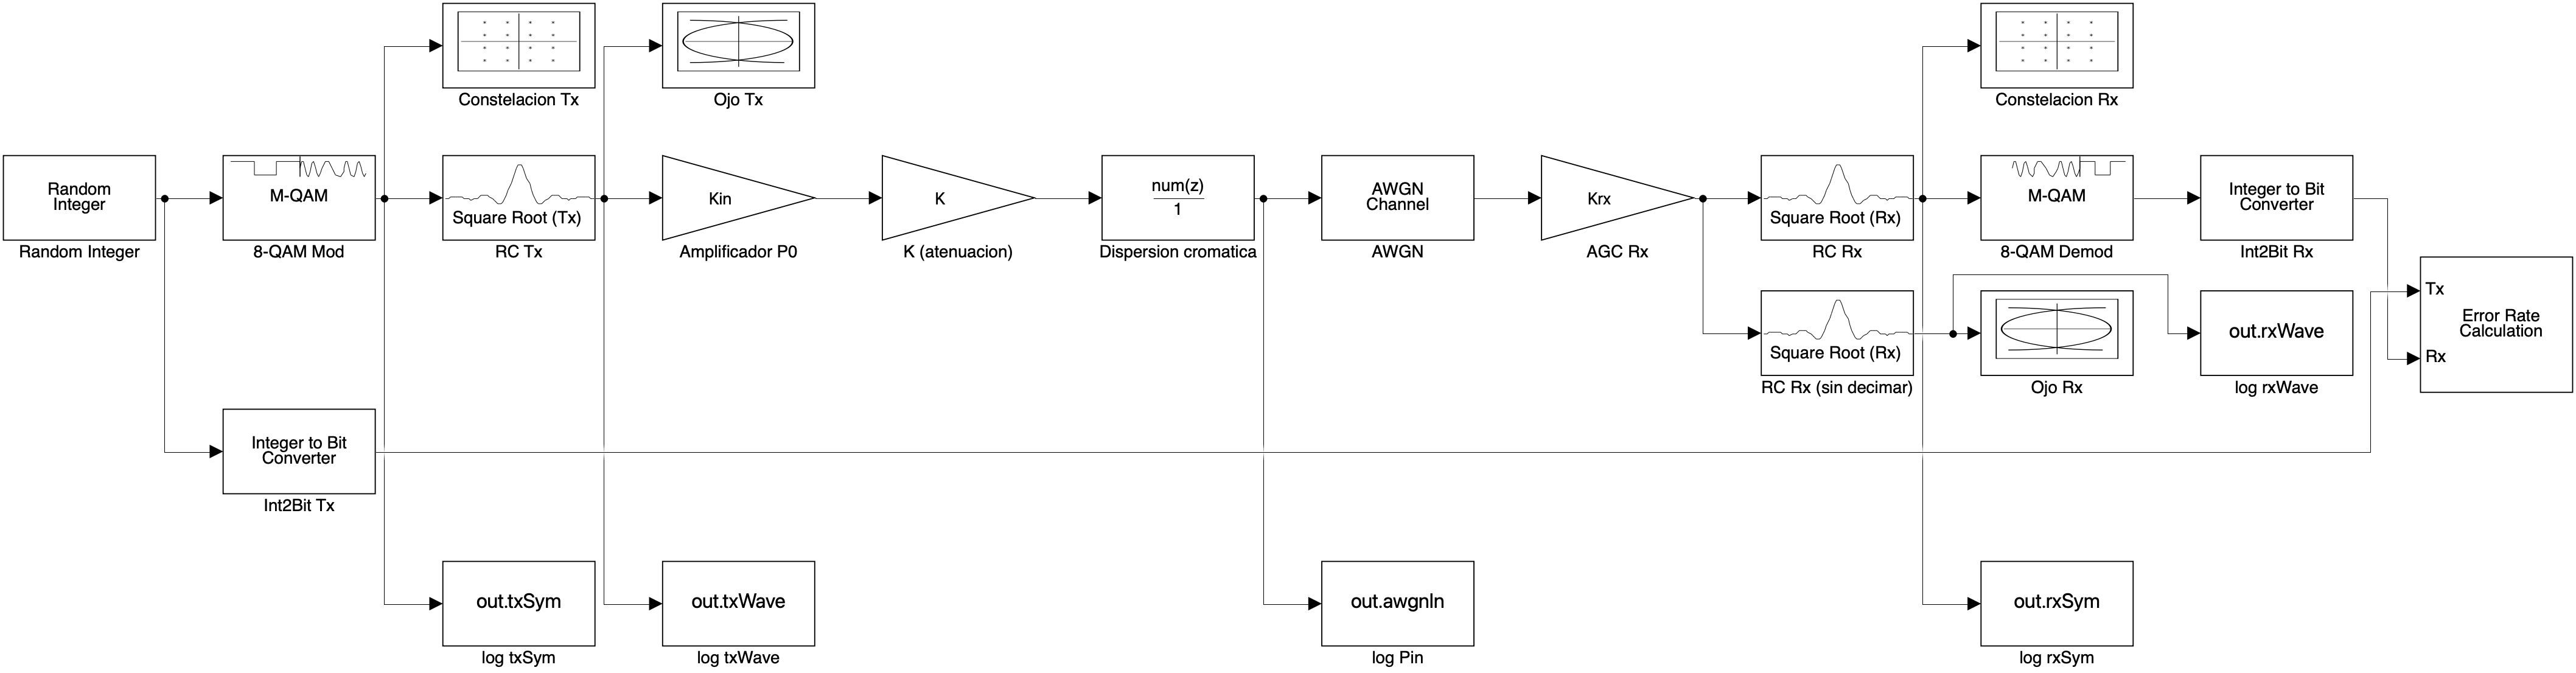
\includegraphics[width=\textwidth]{00_diagrama_bloques.png}
\caption{Modelo Simulink \texttt{enlace\_fibra\_8QAM.slx}.}\label{fig:bloques}
\end{figure}

\begin{itemize}\setlength\itemsep{1pt}
\item \textbf{Transmisor:} \textit{Random Integer Generator} ($M=8$, tramas de 300 símbolos) $\to$ \textit{Rectangular QAM Modulator} ($M=8$, potencia media \SI{1}{W}) $\to$ \textit{Raised Cosine Transmit Filter} (RRC). El bloque ``Amplificador P0'' escala la potencia de transmisión y vale 1 en el caso base.
\item \textbf{Canal:} \textit{Gain} $K$ $\to$ \textit{Discrete FIR Filter} con $H_{CD}(f)$: 256 coeficientes complejos obtenidos por IFFT. Si la dispersión está desactivada, el FIR es un retardo puro de 128 muestras, para conservar la alineación. Luego viene el \textit{AWGN Channel} en modo $E_b/N_0$, con 3 bits/símbolo, 8 muestras/símbolo y potencia de entrada \SI{0.0125}{W}.
\item \textbf{Receptor:} AGC (ganancia $1/K$, equivalente al preamplificador del receptor) $\to$ \textit{Raised Cosine Receive Filter} (RRC, diezmado $\times8$) $\to$ \textit{Rectangular QAM Demodulator} $\to$ \textit{Integer to Bit Converter}.
\item \textbf{Medición:} \textit{Error Rate Calculation} compara los bits transmitidos con los recibidos, con un retardo de 78 bits. Guarda $[\text{BER},\text{errores},\text{bits}]$ en la variable \texttt{BER} y detiene la simulación al alcanzar \texttt{maxNumErrs} errores o \texttt{maxNumBits} bits, lo que lo hace compatible con la pestaña Monte Carlo de \texttt{bertool}. Se incluyen \textit{Constellation Diagram} a la salida del modulador y a la entrada del demodulador, y \textit{Eye Diagram} a la salida de los filtros Tx y Rx.
\end{itemize}

\textbf{Validación.} Sin ruido ($E_b/N_0=\SI{100}{dB}$), la BER fue exactamente 0 en $3\cdot10^5$ bits. La potencia medida a la entrada del AWGN (\SI{0.01251}{W}) coincide con la calculada. La correlación cruzada entre los símbolos transmitidos y los recibidos confirmó el retardo de 26 símbolos.

\section{Resultados}
\subsection{Diagrama de constelación}
El diagrama de constelación representa cada símbolo en el plano complejo: la componente en fase (I) en abscisas y la de cuadratura (Q) en ordenadas, con una muestra por símbolo. En el transmisor muestra los 8 puntos ideales: 4 niveles en I ($\pm0{,}41$, $\pm1{,}22$) por 2 en Q ($\pm0{,}41$). En el receptor permite medir, visualmente o mediante EVM/MER, distintas degradaciones:
\begin{itemize}\setlength\itemsep{1pt}
\item el ruido, por la dispersión de las nubes;
\item la ISI, por la deformación de las nubes;
\item los errores de ganancia, porque la constelación aparece escalada;
\item los errores de fase o frecuencia, porque aparece rotada;
\item los errores de sincronismo.
\end{itemize}

\begin{figure}[H]\centering
\begin{subfigure}{0.24\textwidth}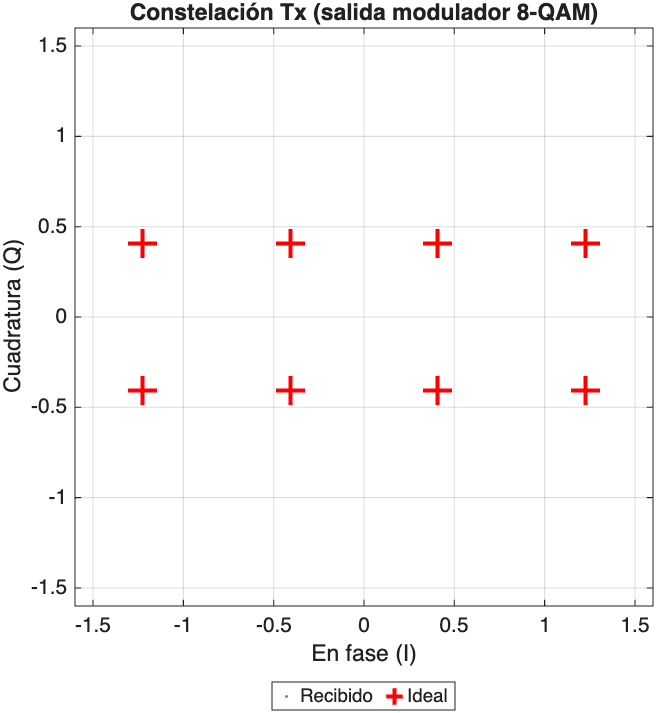
\includegraphics[width=\linewidth]{01_const_tx.png}\caption{Tx}\end{subfigure}
\begin{subfigure}{0.24\textwidth}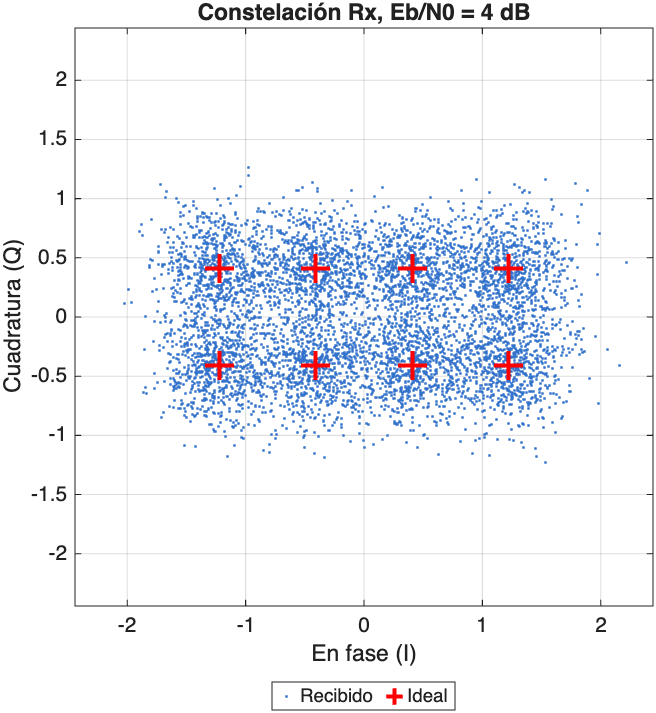
\includegraphics[width=\linewidth]{02_const_rx_04dB.png}\caption{Rx, \SI{4}{dB}}\end{subfigure}
\begin{subfigure}{0.24\textwidth}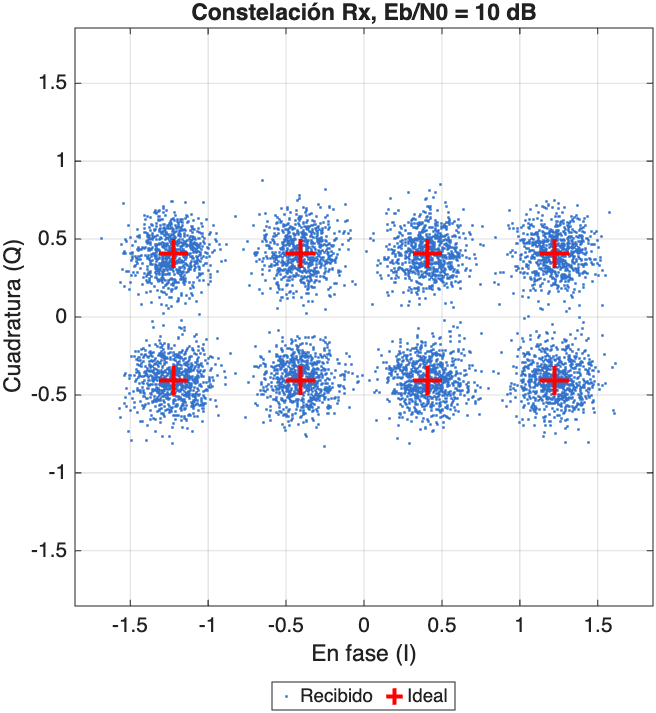
\includegraphics[width=\linewidth]{02_const_rx_10dB.png}\caption{Rx, \SI{10}{dB}}\end{subfigure}
\begin{subfigure}{0.24\textwidth}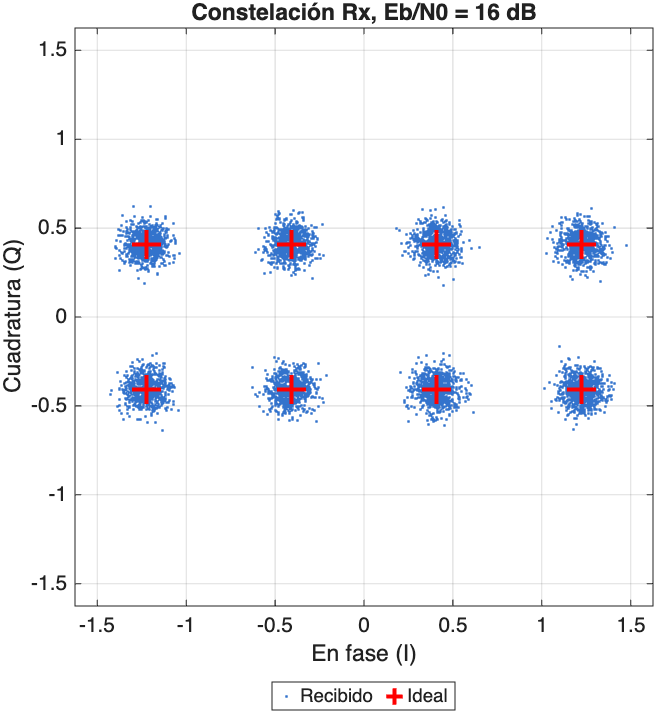
\includegraphics[width=\linewidth]{02_const_rx_16dB.png}\caption{Rx, \SI{16}{dB}}\end{subfigure}
\caption{Constelación a la salida del modulador y a la entrada del demodulador para varios $E_b/N_0$.}\label{fig:const}
\end{figure}

A la salida del modulador, los símbolos coinciden con los puntos ideales. A la entrada del demodulador, cada punto se convierte en una nube circular, lo que indica ruido aditivo gaussiano sin ISI ni distorsión de fase, gracias al filtro adaptado RRC--RRC y al AGC.
\begin{itemize}\setlength\itemsep{1pt}
\item A \SI{4}{dB} las nubes se superponen y aparecen errores de decisión (BER $\approx4{,}7\cdot10^{-2}$).
\item A \SI{10}{dB} están separadas, salvo colas ocasionales (BER $\approx7\cdot10^{-4}$).
\item A \SI{16}{dB} son compactas.
\end{itemize}
Las nubes conservan su posición, lo que confirma que la atenuación de \SI{10}{dB} quedó bien compensada.

\subsection{Diagrama de ojo}
El diagrama de ojo superpone segmentos de la forma de onda de dos símbolos de duración, sincronizados con el reloj de símbolo. De él se obtiene:
\begin{itemize}\setlength\itemsep{1pt}
\item la apertura vertical, que indica el margen frente al ruido;
\item la apertura horizontal, que indica la tolerancia al jitter;
\item el punto de máxima apertura, que marca el instante óptimo de muestreo;
\item el cierre del ojo, que evidencia ISI.
\end{itemize}
En 8-QAM la rama I tiene 4 niveles (3 ojos) y la rama Q tiene 2 niveles (1 ojo).

\begin{figure}[H]\centering
\begin{subfigure}{0.49\textwidth}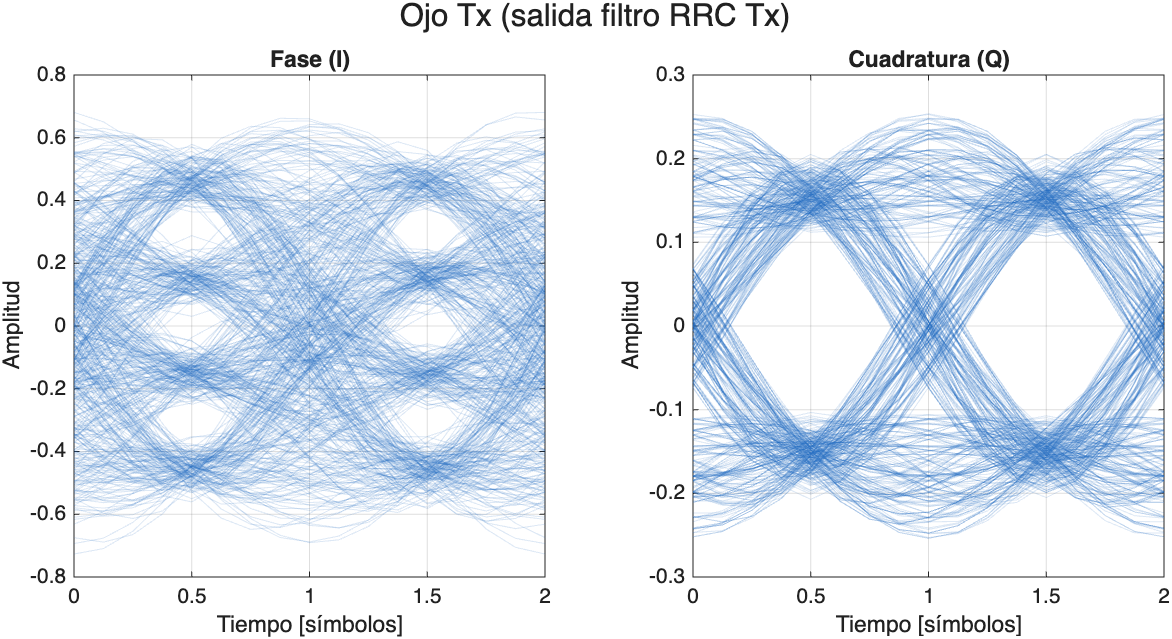
\includegraphics[width=\linewidth]{03_ojo_tx.png}\caption{Salida filtro Tx}\end{subfigure}
\begin{subfigure}{0.49\textwidth}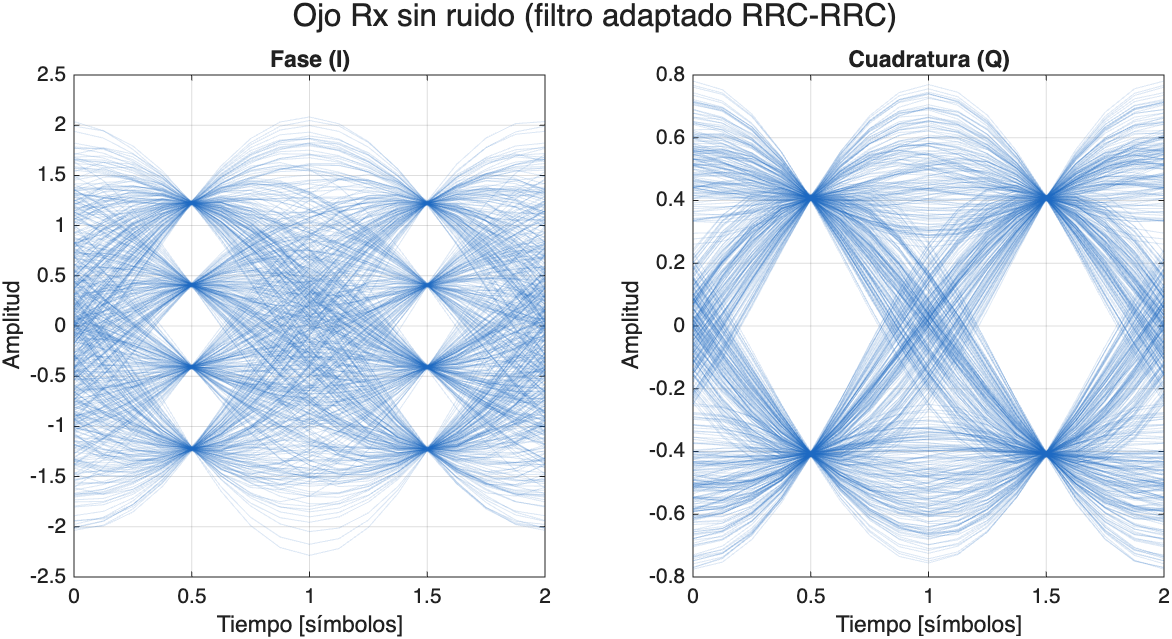
\includegraphics[width=\linewidth]{04_ojo_rx_sin_ruido.png}\caption{Salida filtro Rx, sin ruido}\end{subfigure}\\
\begin{subfigure}{0.49\textwidth}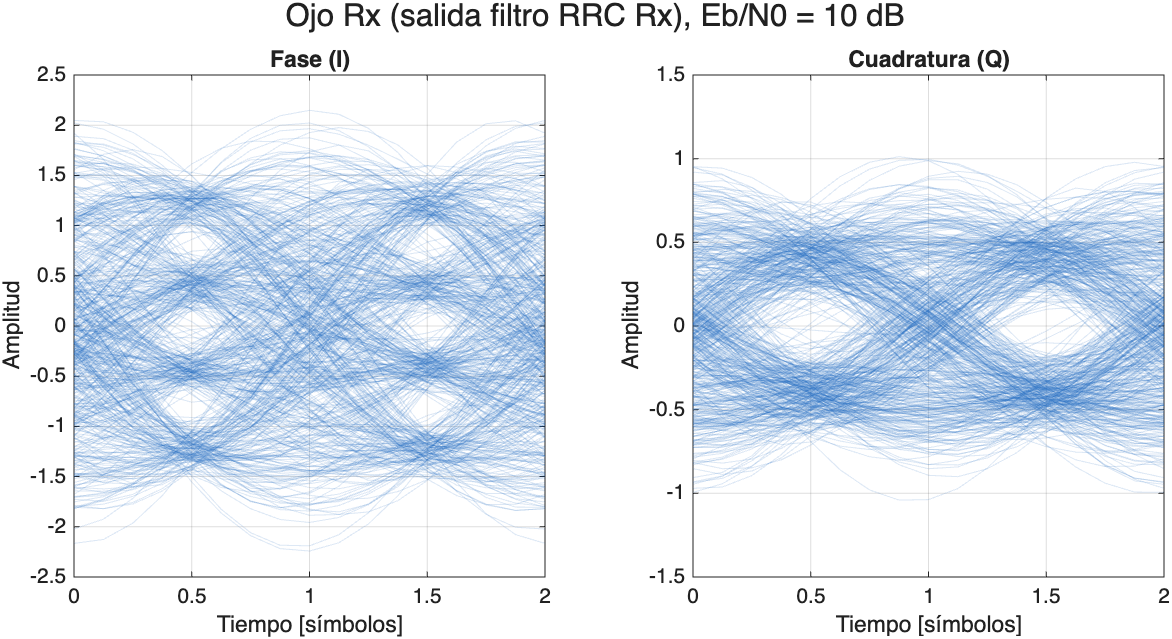
\includegraphics[width=\linewidth]{04_ojo_rx_10dB.png}\caption{Salida filtro Rx, \SI{10}{dB}}\end{subfigure}
\begin{subfigure}{0.49\textwidth}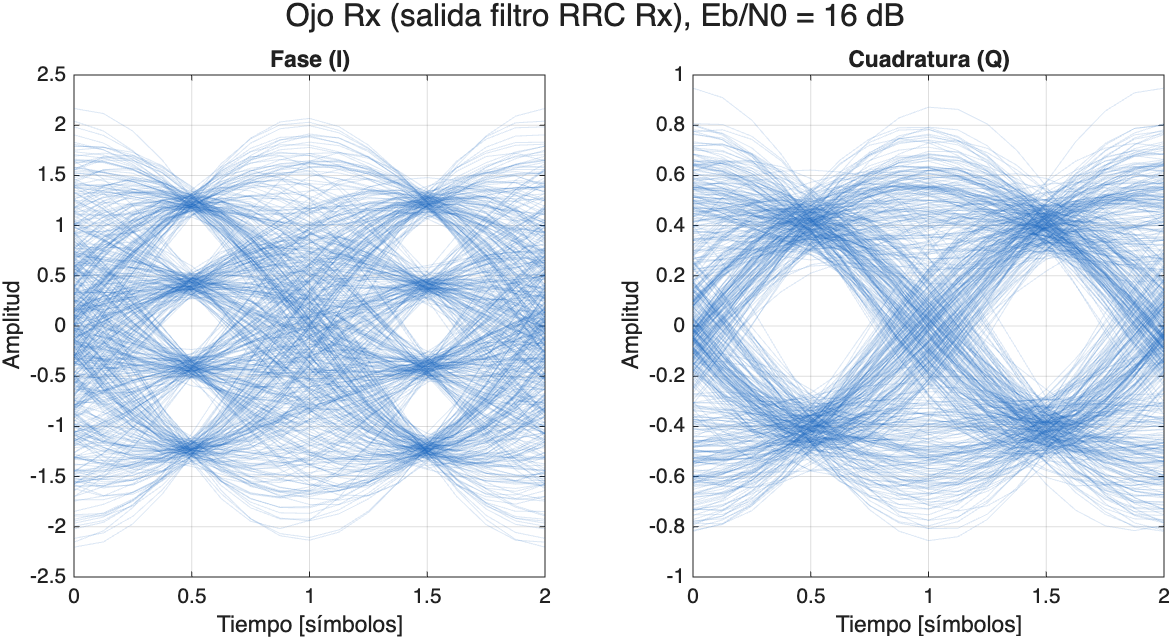
\includegraphics[width=\linewidth]{04_ojo_rx_16dB.png}\caption{Salida filtro Rx, \SI{16}{dB}}\end{subfigure}
\caption{Diagramas de ojo a la salida de los filtros transmisor y receptor.}\label{fig:ojo}
\end{figure}

A la salida del filtro Tx el ojo aparece parcialmente cerrado, porque un único filtro raíz de coseno alzado no cumple el criterio de Nyquist y hay ISI en el instante de muestreo. Tras el filtro Rx, la cascada RRC$\cdot$RRC equivale a un coseno alzado completo. El ojo se abre y las trayectorias convergen en un punto en el instante óptimo ($t=0{,}5$), es decir, la ISI es nula. Con ruido el ojo se cierra verticalmente; a \SI{10}{dB} los cruces se ensanchan pero el ojo sigue abierto, coherente con una BER baja. La rama Q tiene mayor apertura relativa que la I, por lo que la mayoría de los errores ocurren entre niveles de la rama I.

\subsection{BER vs $E_b/N_0$ (\texttt{bertool})}
\begin{figure}[H]\centering
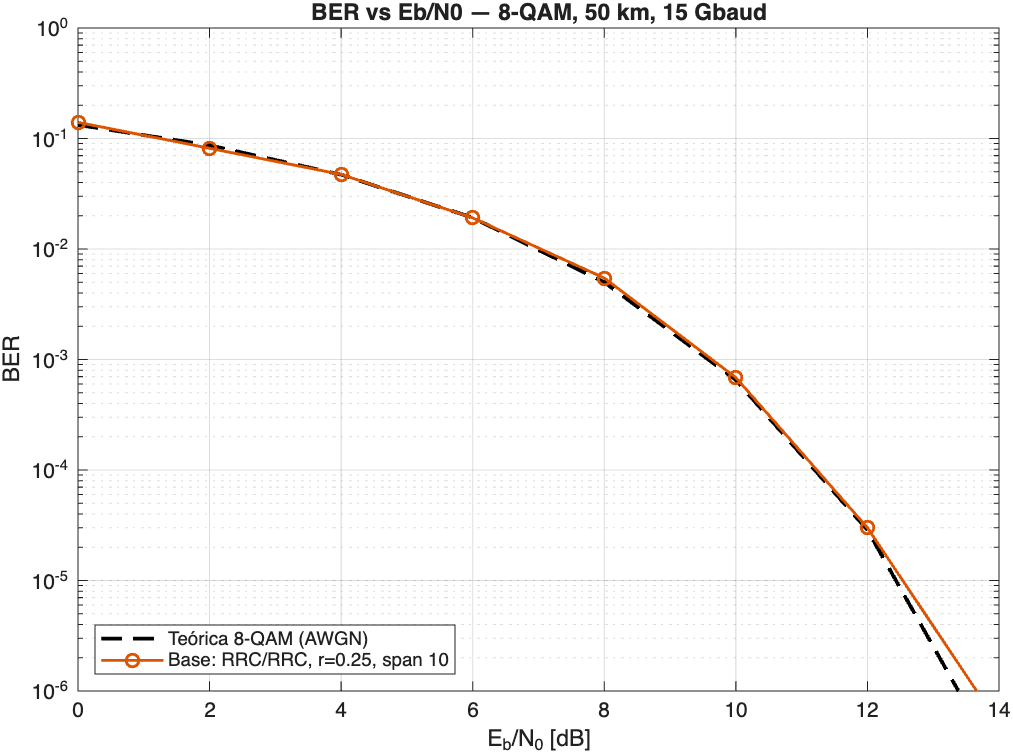
\includegraphics[width=0.6\textwidth]{05_ber_base.png}
\caption{BER simulada (hasta 200 errores o $2\cdot10^6$ bits por punto) y teórica.}\label{fig:ber}
\end{figure}
\begin{table}[H]\centering\small
\caption{BER teórica y simulada del caso base.}
\begin{tabular}{lcccccccc}\toprule
$E_b/N_0$ [dB] & 0 & 2 & 4 & 6 & 8 & 10 & 12 & 14\\\midrule
Teórica & 1,3e-1 & 8,7e-2 & 4,7e-2 & 1,9e-2 & 5,0e-3 & 6,5e-4 & 2,9e-5 & 2,3e-7\\
Simulada & 1,4e-1 & 8,2e-2 & 4,7e-2 & 1,9e-2 & 5,5e-3 & 6,9e-4 & 3,0e-5 & 5,0e-7\\\bottomrule
\end{tabular}\end{table}

La curva simulada se superpone a la teórica de 8-QAM en AWGN. La única diferencia apreciable está a \SI{14}{dB}: con $2\cdot10^6$ bits se observó un solo error, de modo que el estimador no es confiable a ese nivel. Para alcanzar BER $=10^{-3}$ (umbral típico antes de FEC), el enlace requiere $E_b/N_0\approx\SI{9.6}{dB}$. Como $E_b/N_0$ es una magnitud relativa, el resultado no depende de la potencia absoluta.

\section{Modificaciones y análisis}
Se mantuvieron la modulación 8-QAM y la longitud de \SI{50}{km}, y se realizaron ocho modificaciones, incluida la dispersión cromática opcional (tabla~\ref{tab:mods}).

\begin{table}[H]\centering\small
\caption{Resumen de las modificaciones.}\label{tab:mods}
\begin{tabular}{llcl}\toprule
\# & Modificación & BER @\SI{10}{dB} & Efecto\\\midrule
--- & Base (RRC/RRC, $r=0{,}25$, span 10) & 6,9e-4 & coincide con la teoría\\
M1 & Tx Normal + Rx RRC (fig.~1 del enunciado) & 2,1e-3 & $\approx\SI{1.2}{dB}$ de penalidad a $10^{-3}$\\
M2a & Roll-off 0,05 & 3,8e-3 & $\approx\SI{2.5}{dB}$ de penalidad\\
M2b & Roll-off 0,9 & 7,6e-4 & sin penalidad; BW \SI{28.5}{GHz} vs \SI{18.75}{GHz}\\
M3 & Span 2 símbolos & 4,7e-2 & piso de error $\approx4\cdot10^{-2}$\\
M4 & Retardo erróneo (+1 bit) & 0,52 & bits desalineados\\
M5 & Sin AGC en el receptor & 0,18 & constelación escalada por 0,32\\
M6 & 2 muestras/símbolo & 7,0e-4 & BER igual; ojo pobremente muestreado\\
M7 & Potencia Tx \SI{10}{W} & 6,2e-4 & BER igual: $E_b/N_0$ es relativo\\
M8 & Dispersión cromática & 0,14 & piso $\approx0{,}15$ sin ecualizar\\\bottomrule
\end{tabular}\end{table}

\begin{figure}[H]\centering
\begin{subfigure}{0.48\textwidth}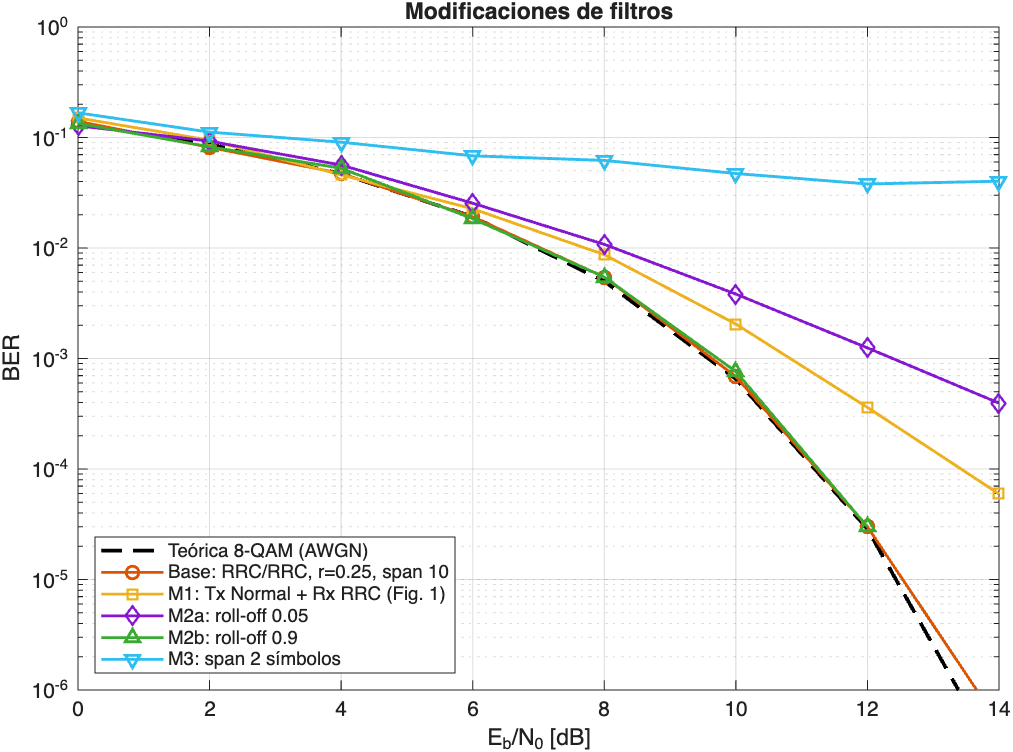
\includegraphics[width=\linewidth]{06_ber_filtros.png}\caption{Filtros (M1--M3)}\end{subfigure}
\begin{subfigure}{0.48\textwidth}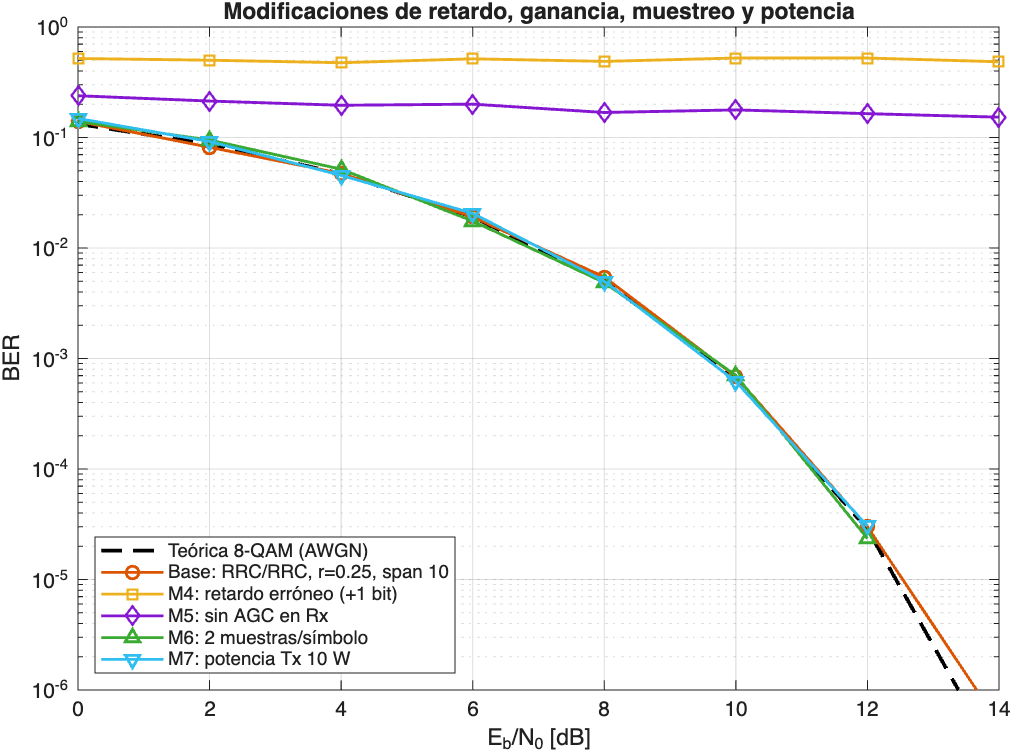
\includegraphics[width=\linewidth]{07_ber_otros.png}\caption{Retardo, ganancia, muestreo y potencia (M4--M7)}\end{subfigure}
\caption{BER vs $E_b/N_0$ para las modificaciones.}\label{fig:bermods}
\end{figure}
\begin{figure}[H]\centering
\begin{subfigure}{0.49\textwidth}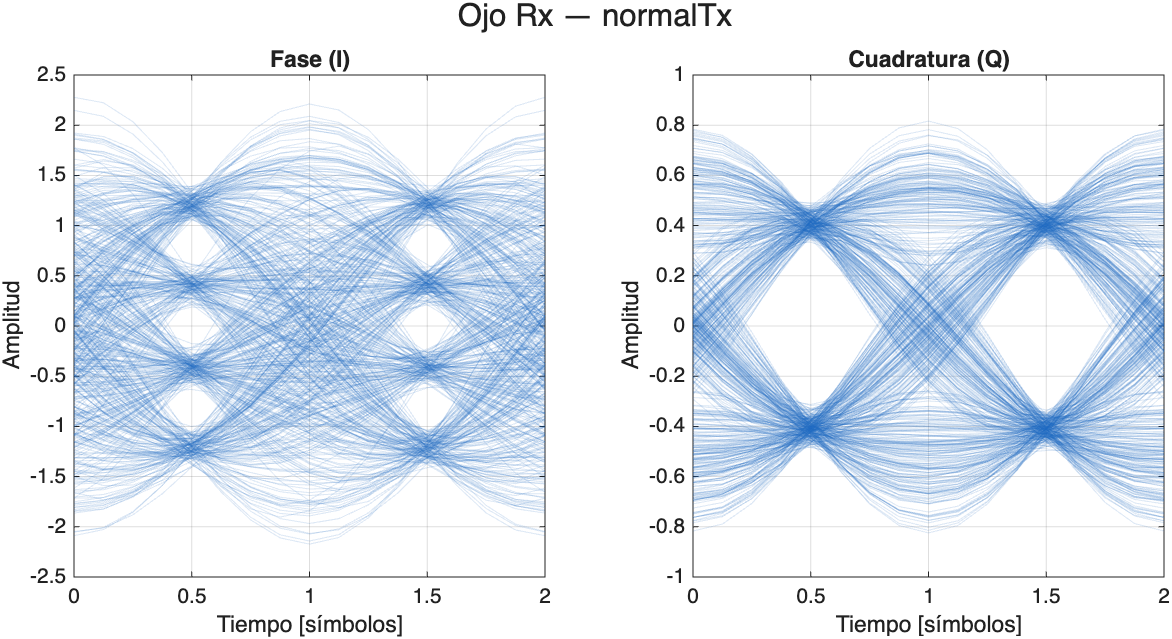
\includegraphics[width=\linewidth]{m_normalTx_ojo_rx.png}\caption{M1: Tx Normal}\end{subfigure}
\begin{subfigure}{0.49\textwidth}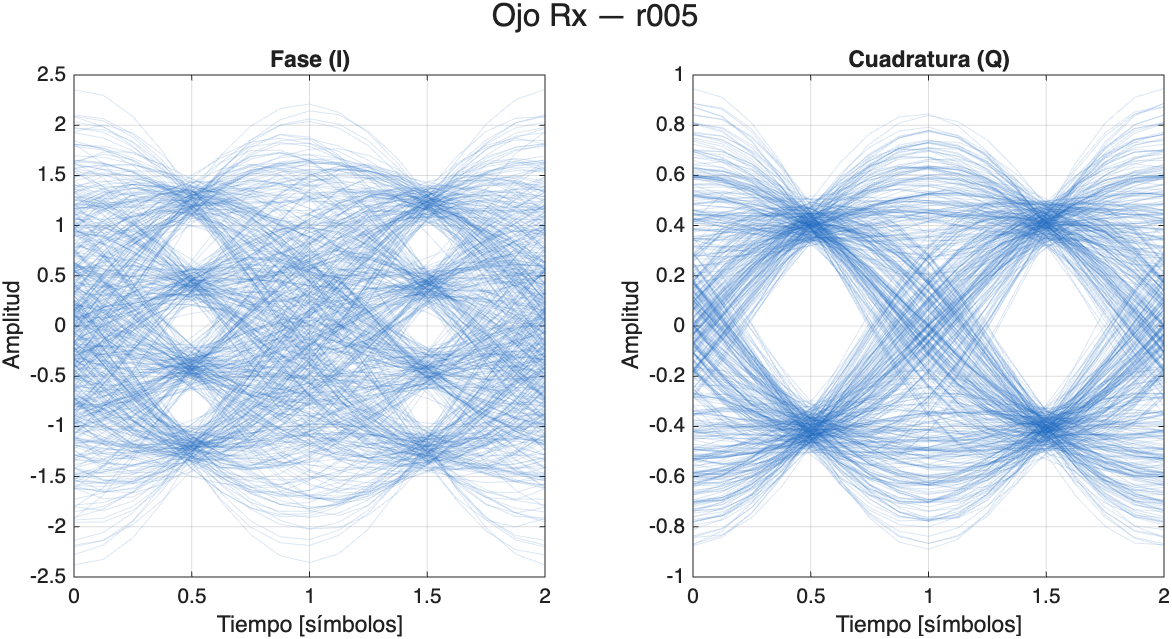
\includegraphics[width=\linewidth]{m_r005_ojo_rx.png}\caption{M2a: $r=0{,}05$}\end{subfigure}\\
\begin{subfigure}{0.49\textwidth}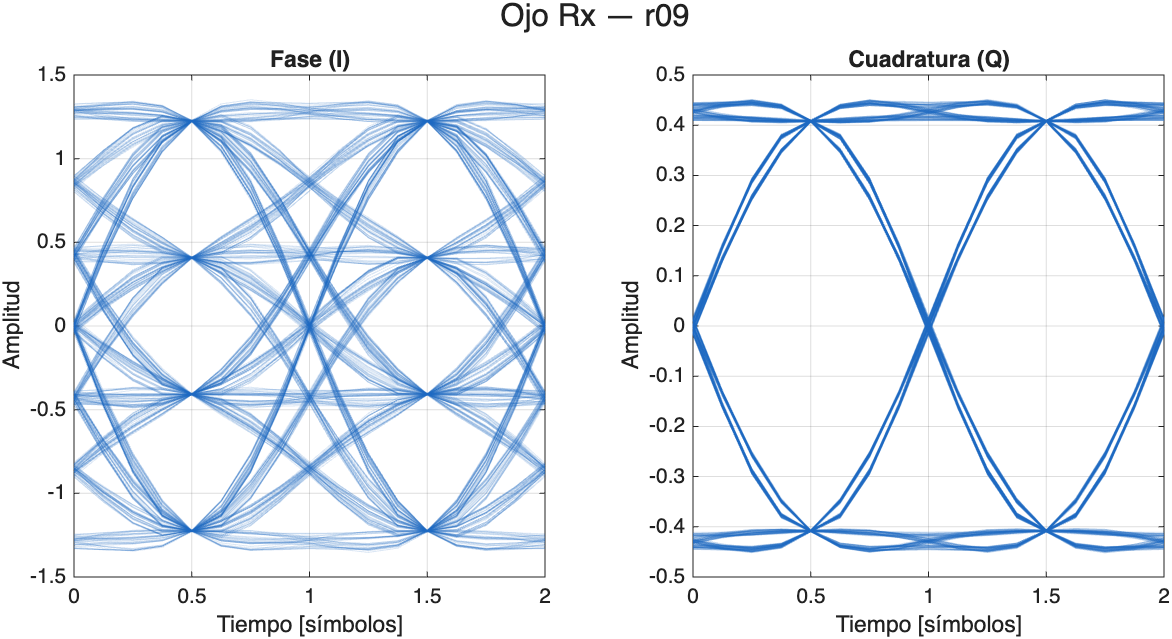
\includegraphics[width=\linewidth]{m_r09_ojo_rx.png}\caption{M2b: $r=0{,}9$}\end{subfigure}
\begin{subfigure}{0.49\textwidth}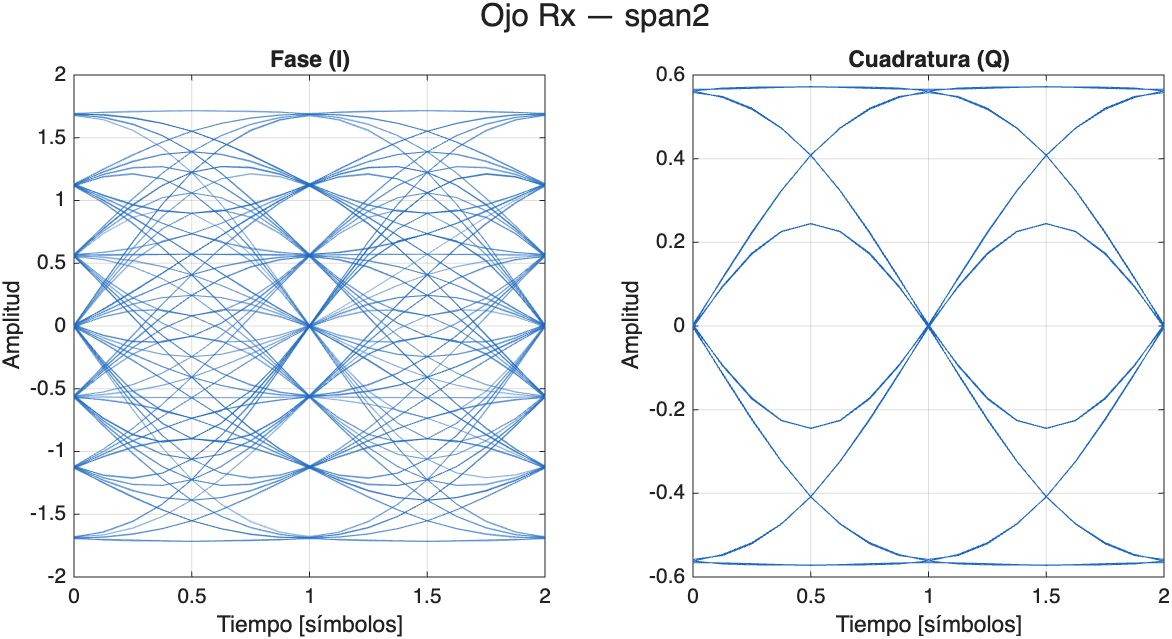
\includegraphics[width=\linewidth]{m_span2_ojo_rx.png}\caption{M3: span 2}\end{subfigure}
\caption{Ojo a la salida del filtro Rx, sin ruido, para las modificaciones de filtros.}\label{fig:ojomods}
\end{figure}

\textbf{M1 -- Filtro Normal en Tx y raíz en Rx.} La respuesta total (coseno alzado por raíz) no es de Nyquist, y el filtro Rx deja de estar adaptado. En el ojo, las trayectorias no convergen a un punto. La penalidad crece con $E_b/N_0$ ($\approx\SI{1.2}{dB}$ a $10^{-3}$ y $\approx\SI{2.5}{dB}$ a $10^{-4}$), porque la ISI es determinística y domina cuando el ruido es pequeño. Por eso se adoptó RRC--RRC como caso base.

\textbf{M2 -- Roll-off.}
\begin{itemize}\setlength\itemsep{1pt}
\item Con $r=0{,}05$, el ancho de banda baja a \SI{15.75}{GHz}, pero el pulso decae lentamente y el span de 10 lo trunca. Esto genera ISI y un ojo con apertura horizontal casi nula, de máxima sensibilidad al jitter, con una penalidad de $\approx\SI{2.5}{dB}$.
\item Con $r=0{,}9$, la BER es la teórica, pero el enlace ocupa \SI{28.5}{GHz} (+52\,\%), lo que reduce la cantidad de canales en DWDM.
\end{itemize}
$r=0{,}25$ es un buen compromiso.

\textbf{M3 -- Span de 2 símbolos.} Con solo 17 coeficientes, los filtros no son de Nyquist ni adaptados. Incluso sin ruido, en el instante de muestreo (desplazado a $t=1$ por el menor retardo) la rama I converge a 7 niveles en lugar de 4 y la Q a 3 en lugar de 2, porque la ISI fusiona niveles vecinos. La BER se estanca en $\approx4\cdot10^{-2}$, un piso que no se corrige aumentando la potencia.

\textbf{M4 -- Retardo.} Desplazar en un bit el retardo de \textit{Error Rate Calculation} hace que se comparen bits no correspondientes, y la BER es $\approx0{,}5$ para cualquier $E_b/N_0$. La sincronización es tan crítica como la SNR.

\begin{figure}[H]\centering
\begin{subfigure}{0.3\textwidth}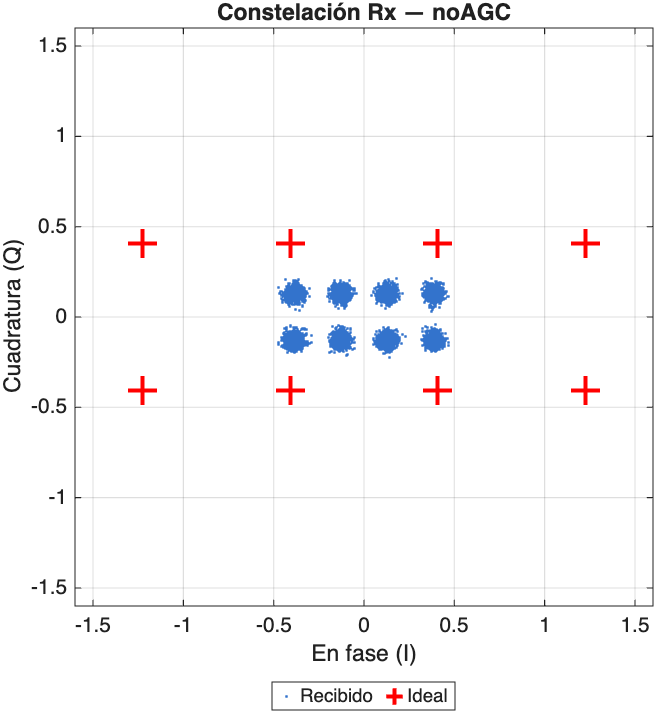
\includegraphics[width=\linewidth]{m_noAGC_const_rx.png}\caption{M5: sin AGC, \SI{14}{dB}}\end{subfigure}
\begin{subfigure}{0.3\textwidth}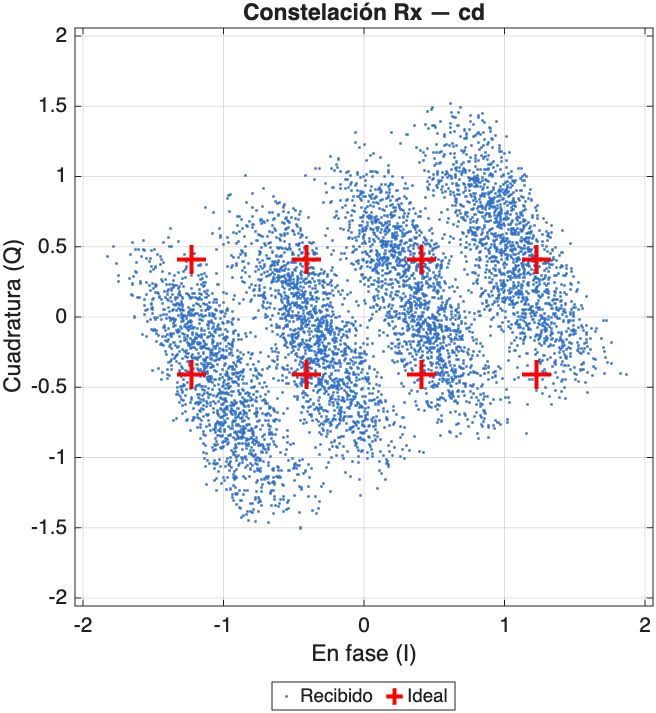
\includegraphics[width=\linewidth]{m_cd_const_rx.png}\caption{M8: con CD, sin ruido}\end{subfigure}
\begin{subfigure}{0.36\textwidth}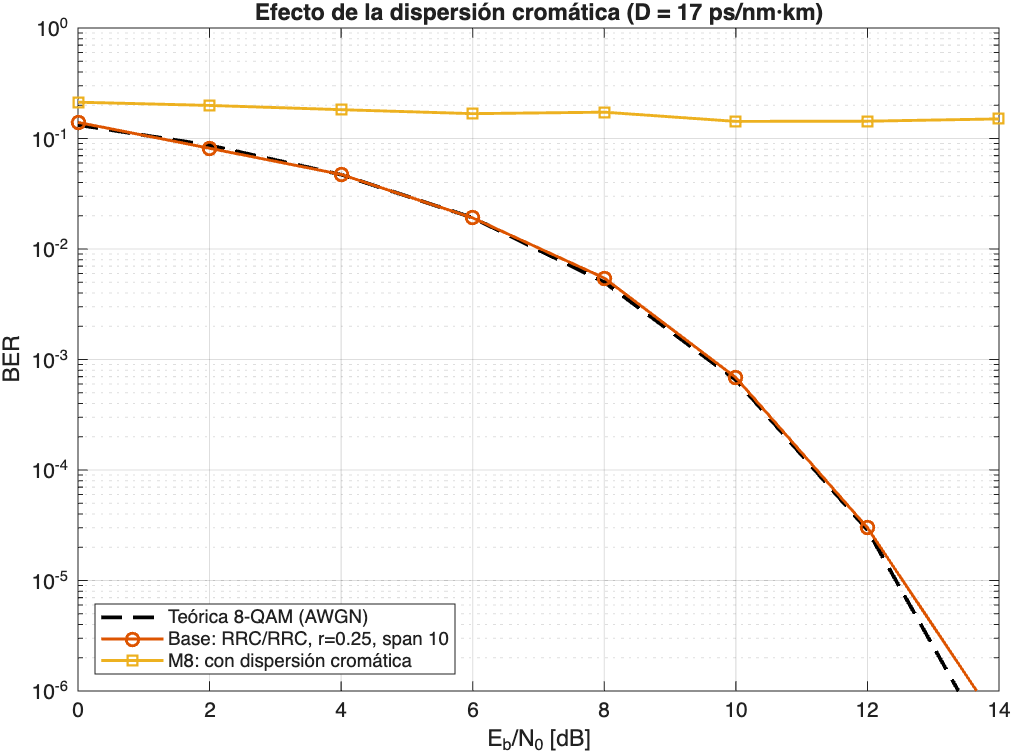
\includegraphics[width=\linewidth]{08_ber_cd.png}\caption{M8: BER con y sin CD}\end{subfigure}
\caption{Constelaciones en el receptor sin AGC y con dispersión cromática.}\label{fig:agccd}
\end{figure}

\textbf{M5 -- Sin AGC.} La señal llega con $\sqrt{0{,}1}=0{,}32$ veces la amplitud esperada. El demodulador usa umbrales para \SI{1}{W} y decide todos los símbolos como de las columnas interiores, por lo que la BER queda entre 0,15 y 0,2. En QAM la amplitud porta información, así que el control de ganancia del receptor (o un amplificador óptico) es indispensable.

\textbf{M6 -- 2 muestras/símbolo.} La BER no cambia, porque las decisiones dependen solo de la muestra óptima y el AWGN referencia la potencia por símbolo. Sin embargo, los ojos pierden resolución y la simulación representa peor la forma de onda analógica.

\textbf{M7 -- Potencia de \SI{10}{W}.} La BER es idéntica, porque el bloque AWGN ajusta el ruido para mantener el $E_b/N_0$ pedido. En un enlace real, más potencia sí mejora la SNR, hasta que aparecen efectos no lineales (Kerr), que no se modelan aquí.

\textbf{M8 -- Dispersión cromática.} Aunque $L=\SI{50}{km}<L_D\approx\SI{205}{km}$, el ensanchamiento de $\approx1{,}9$ símbolos mezcla cada símbolo con sus vecinos. Sin ruido, la constelación se convierte en nubes deformadas y rotadas, y la BER se estanca en $\approx0{,}15$ con independencia de $E_b/N_0$. Como $H_{CD}$ es de fase pura, un ecualizador digital $H_{CD}^*(f)=e^{+j2\pi^2\beta_2Lf^2}$ en un receptor coherente la eliminaría por completo. En un sistema IM/DD, en cambio, la dispersión produciría desvanecimiento selectivo en frecuencia, que no se compensa linealmente.

\section{Conclusiones}
\begin{itemize}\setlength\itemsep{1pt}
\item El modelo reproduce la BER teórica de 8-QAM en AWGN (BER $=10^{-3}$ a $E_b/N_0\approx\SI{9.6}{dB}$). Esto valida la atenuación ($G_a=0{,}1$), la calibración de potencia del AWGN (\SI{0.0125}{W}/muestra) y el retardo de 78 bits.
\item La atenuación de \SI{10}{dB} es transparente para la BER siempre que el receptor recupere la escala de amplitud. Sin control de ganancia, la detección 8-QAM falla (BER $\approx0{,}15$).
\item Los filtros deben formar un par adaptado RRC--RRC con span suficiente. La configuración Normal--raíz cuesta entre 1 y \SI{2.5}{dB}, y los spans cortos o roll-off muy bajos generan ISI y pisos de error. El roll-off fija el compromiso entre ancho de banda, $15(1+r)$~GHz, y robustez.
\item Los diagramas de constelación y de ojo permiten diagnosticar el tipo de degradación, complementando la curva BER:
\begin{itemize}\setlength\itemsep{0pt}
\item ruido: nubes circulares y ojo cerrado verticalmente;
\item ISI: nubes deformadas y cruces que no convergen;
\item error de ganancia: constelación escalada.
\end{itemize}
\item La dispersión cromática a \SI{1550}{nm} produce, en \SI{50}{km} a \SI{15}{Gbaud}, una ISI de unos 2 símbolos que vuelve inutilizable el enlace sin compensación. En la práctica se corrige con DSP en receptores coherentes o con fibra compensadora.
\end{itemize}

\noindent\textbf{Archivos entregados:} \texttt{enlace\_fibra\_8QAM.slx} (modelo); \texttt{init\_params.m} e \texttt{init\_derived.m} (parámetros, cargados en \textit{InitFcn}); \texttt{build\_model.m} (construcción del modelo); \texttt{run\_all.m} (barridos y figuras).

\end{document}
